\begin{frame}
      \frametitle{Satisfiability Solving: A Success Story}
      \begin{itemize}
            \item Satisfiability solvers~\cite{SATHandbook} have succeeded in various fields
                  \begin{itemize}
                        \item Artificial intelligence~\cite{Nilsson2014,Russell2020}
                        \item Electronic design automation~\cite{Marques2000,Wang2009}
                        \item Formal verification~\cite{Berard2013,Jhala2009}
                  \end{itemize}
      \end{itemize}
\end{frame}

\begin{frame}
      \frametitle{Satisfiability beyond Propositional Logic}
      \begin{figure}
            \centering
            \begin{frame}
  \frametitle{Complexity}
  \begin{block}{Theorem: NEXPTIME-Completeness of DSSAT}
    The decision version of DSSAT is NEXPTIME-complete
    \pause
    \begin{itemize}
      \item DSSAT is NEXPTIME
            \pause
      \item DSSAT is NEXPTIME-hard
    \end{itemize}
  \end{block}
  \pause
  \begin{block}{Proof Sketch}
    \belowdisplayskip=0pt
    \begin{itemize}
      \item NEXPTIME
            \pause
            \begin{enumerate}
              \item nondeterministically construct a set of Skolem functions $\skf$
                    \pause
              \item compute $\spb{\pcf{\Qf}{\skf}}$ and compare it with the threshold $\theta$
            \end{enumerate}
            \pause
      \item NEXPTIME-hard: DQBF $\leq_P$ DSSAT
            \pause
            \begin{align*}
              \Qf_Q=\forall x_1, \ldots, \forall x_n, \exists y_1(D_{y_1}), \ldots, \exists y_m(D_{y_m}).\pf
            \end{align*}
            \pause
            \begin{align*}
              \Qf_S=\random{0.5} x_1, \ldots, \random{0.5} x_n, \exists y_1(D_{y_1}), \ldots, \exists y_m(D_{y_m}).\pf
            \end{align*}
            \pause
            Claim: $\Qf_Q$ is satisfiable if and only if $\spb{\pcf{\Qf_S}{\skf}} \geq 1$ for some $\skf$
    \end{itemize}
  \end{block}
\end{frame}
      \end{figure}
\end{frame}

\begin{frame}
      \frametitle{This Dissertation in a Nutshell}
      \begin{figure}
            \centering
            \documentclass{standalone}
\usepackage{tikz}
\begin{document}
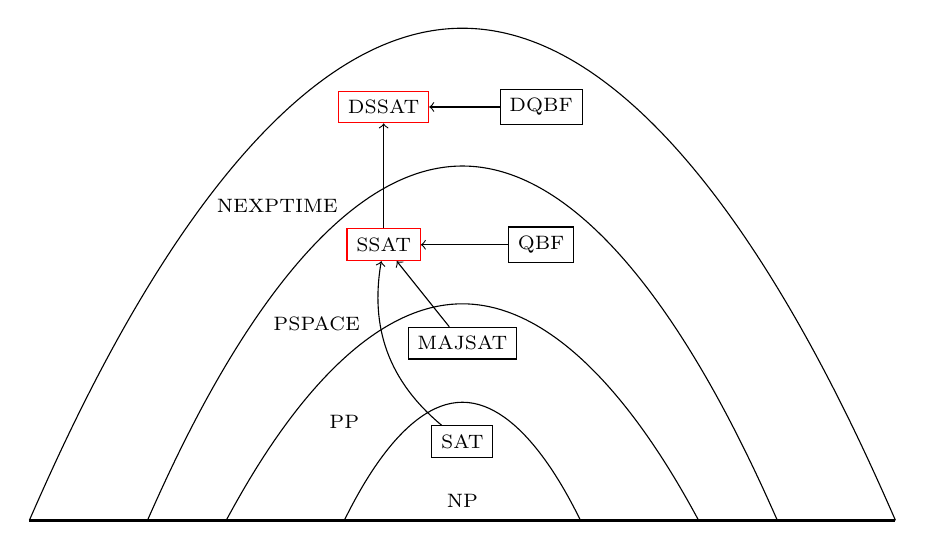
\begin{tikzpicture}[auto]
    \tikzstyle{every node}=[font=\scriptsize]
    \pgftransformscale{.5}
    %%% HELP LINES - uncomment to design/extend
    %\draw[step=1cm,gray,very thin] (-10,0) grid (10,12);
    %\node at (0,0) {\textbf{(0,0)}};
    %% Horizontal bar
    \draw[very thick] (-11,0) -- (11,0);
    % NP
    \draw (-3,0) parabola bend (0,3) (3,0);
    \node at (0,0.5) {NP};
    \node at (0,2) [draw,rectangle] (SAT) {SAT};
    % PP
    \draw (-6,0) parabola bend (0,5.5) (6,0);
    \node at (-3,2.5) {PP};
    \node at (0,4.5) [draw,rectangle] (MAJSAT) {MAJSAT};
    % PSPACE
    \draw (-8,0) parabola bend (0,9) (8,0);
    \node at (-3.7,5) {PSPACE};
    \node at (2,7) [draw,rectangle] (QBF) {QBF};
    \node at (-2,7) [draw=red,rectangle] (SSAT) {SSAT};
    % NEXPTIME
    \draw (-11,0) parabola bend (0,12.5) (11,0);
    \node at (-4.7,8) {NEXPTIME};
    \node at (2,10.5) [draw,rectangle] (DQBF) {DQBF};
    \node at (-2,10.5) [draw=red,rectangle] (DSSAT) {DSSAT};

    \path
    (SAT) edge [->,bend left] (SSAT)
    (MAJSAT) edge [->] (SSAT)
    (QBF) edge [->] (SSAT)
    (SSAT) edge [->] (DSSAT)
    (DQBF) edge [->] (DSSAT);
\end{tikzpicture}
\end{document}
      \end{figure}
\end{frame}

\begin{frame}
      \frametitle{Decision Making under Uncertainty}
      \begin{itemize}
            \item Stochastic Boolean satisfiability (SSAT)
                  \begin{itemize}
                        \item \emph{Games against nature}~\cite{Papadimitriou1985}
                        \item Randomized quantifier $\random{p}x$: $\spb{x=\true}=p$
                        \item Logical formalism for problems with uncertainty
                              \begin{itemize}
                                    \item Probabilistic planning~\cite{Majercik1998,Majercik2003,Majercik2005} and POMDP~\cite{Salmon2020}
                              \end{itemize}
                  \end{itemize}
                  \pause
            \item Application to VLSI systems?
                  \begin{itemize}
                        \item Conventionally: error detection~\cite{Constantinescu2003} or correction~\cite{Mitra2006}
                        \item Post-Moore: probabilistic behavior of devices~\cite{Chakrapani2006ProbDesign}
                  \end{itemize}
      \end{itemize}
\end{frame}

\begin{frame}
      \frametitle{Accepting Device Imperfection}
      \begin{itemize}
            \item New computational paradigms
                  \begin{itemize}
                        \item Approximate design: deterministic deviation
                              \begin{itemize}
                                    \item E.g., neural-network deployment to edge devices
                                    \item Circuit architectures~\cite{Kahng2012,Ye2013,Kim2013}
                                    \item Performance analysis~\cite{Li2014,Venkatesan2011ApproxDesign}
                                    \item Automatic synthesis~\cite{Miao2013,Miao2014,Mrazek2016,Rehman2016,Venkataramani2012}
                              \end{itemize}
                        \item Probabilistic design: nondeterministic deviation
                              \begin{itemize}
                                    \item E.g., low-power video decoding
                                    \item Energy consumption vs. correct switching of probabilistic CMOS~\cite{Chakrapani2006ProbDesign}
                              \end{itemize}
                  \end{itemize}
      \end{itemize}
\end{frame}

\begin{frame}
      \frametitle{Analyzing Probabilistic Design}
      \begin{itemize}
            \item Circuit reliability analysis
                  \begin{itemize}
                        \item Permanent defects or transient faults
                        \item Error probability at primary outputs
                        \item Monte Carlo simulation~\cite{Mohanram2003} or statistical methods~\cite{Bahar2003,Krishnaswamy2005,Rejimon2005}
                        \item Inadequate to analyze probabilistic design
                              \begin{itemize}
                                    \item Single-gate failure
                                    \item Average error rate
                              \end{itemize}
                  \end{itemize}
                  \pause
            \item \alert{Research need: a framework to analyze probabilistic design}
                  \begin{itemize}
                        \item Design space exploration
                        \item Fault-tolerant applications
                        \item Intrinsically probabilistic systems
                        \item SSAT is a suitable logical formalism
                  \end{itemize}
      \end{itemize}
\end{frame}

\begin{frame}
      \frametitle{State-of-the-Art SSAT Solving}
      \begin{itemize}
            \item DPLL search~\cite{Davis1962}
                  \begin{itemize}
                        \item \maxplan~\cite{Majercik1998}: pure variables and unit propagation
                        \item \zander~\cite{Majercik2003}: threshold-pruning heuristics and memorization
                        \item \dcssat~\cite{Majercik2005}: divide-and-conquer (structure of planning problems)
                  \end{itemize}
                  \pause
            \item Knowledge compilation~\cite{Darwiche2002KnowledgeCompilation}
                  \begin{itemize}
                        \item \complan~\cite{Huang2006}: deterministic, decomposable NNF (d-DNNF)~\cite{Darwiche2001,Darwiche2002dDNNF}
                  \end{itemize}
                  \pause
            \item Closely related to model counting (MAJSAT) and QBF
                  \begin{itemize}
                        \item Randomized quantifier: weighted summation of satisfying assignments
                        \item PSPACE-complete~\cite{Stockmeyer1973}: the same as QBF
                  \end{itemize}
                  \pause
            \item \alert{Research need: novel algorithms for SSAT solving}
                  \begin{itemize}
                        \item Leverage advancements of other formalisms
                  \end{itemize}
      \end{itemize}
\end{frame}

\begin{frame}
      \frametitle{Problems beyond PSPACE-Completeness}
      \begin{itemize}
            \item SSAT is limited within PSPACE-completeness
                  \pause
            \item NEXPTIME-complete~\cite{Peterson1979} problems with randomness
                  \begin{itemize}
                        \item E.g., decentralized POMDP (Dec-POMDP)~\cite{Bernstein2002}
                        \item Difficult to obtain succinct encodings using SSAT
                  \end{itemize}
                  \pause
            \item \alert{Research need: modeling NEXPTIME problems with uncertainty}
                  \begin{itemize}
                        \item Extend DQBF to stochastic domain
                  \end{itemize}
      \end{itemize}
\end{frame}

\begin{frame}
      \frametitle{Difficulty in Algorithm Comparison}
      \begin{itemize}
            \item Most SSAT work was done before 2005~\cite{Majercik1998,Majercik2003,Majercik2004,Majercik2005}
                  \begin{itemize}
                        \item Open-source solvers and formula instances are barely available
                  \end{itemize}
                  \pause
            \item \alert{Research need: public SSAT solvers and instances}
                  \begin{itemize}
                        \item Convenient comparison of different algorithms
                  \end{itemize}
      \end{itemize}
\end{frame}